\documentclass[a4paper,11pt]{style-esi/td}

\usepackage{style-esi/licence}	% Affiche une licence dans le document
\usepackage{style-esi/exercice}
\usepackage{style-esi/listing}
\usepackage{style-esi/tutoriel}
\usepackage{style/dev1}
\marginnumbertrue

\newcommand{\findefonctionnalite}{
\begin{infoit}{Fin de fonctionnalité}
	Écrivez la javadoc si ce n'est déjà fait.\\  
	Lorsque votre code est propre, faites un commit avec un nom explicite. 
\end{infoit}
}

\begin{document}

\seance{13}{Mise en pratique~: 3 in line}{td13-inline}{
	Dans ce travail, nous allons développer un jeu simple en essayant de 
	reprendre tous les concepts de ce premier cours de développement. 
	
	Nous mettons en œuvre une approche \textit{tests first} en utilisant JUnit.
	Nous utiliserons des tableaux à une dimension, des structures
	conditionnelles et répétitives. Nous gèrerons nos versions avec
	\textit{git}. Nous prendrons également soin d'écrire la javadoc pour toutes
	nos méthodes.

	\begin{center}
	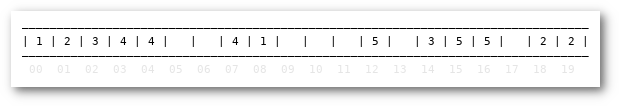
\includegraphics[width=1.05\linewidth]{img/out-3-ombre.png}
	\end{center}
}

\section*{Les règles du jeu}


	Ce jeu se joue seul. Le jeu est constitué d'un plateau pouvant recevoir
	vingt billes de différentes couleurs. Il existe cinq couleurs. Au début du
	jeu, deux billes de couleurs aléatoires sont placées à deux endroits libres
	aléatoires. 
			
	À chaque tour de jeu, le joueur choisit quelle bille déplacer et
	à quelle endroit la déplacer pour peu qu'il n'y ait pas plus d'une
	bille à \textit{sauter}. À chaque déplacement, deux nouvelles billes de
	couleurs aléatoires sont placées à deux endroits libres aléatoires.

	Lorsque trois billes de même couleurs sont alignées côte à côte, elles
	sont supprimées. 

	Le but du jeu est de jouer le plus longtemps possible. 

\bigskip
\bigskip
\subsection*{Exemples}

\textbf{Exemple en fin de partie}

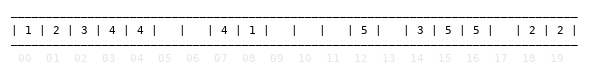
\includegraphics[width=.9\linewidth]{img/out-3.png}

\begin{itemize}

	\item La bille \textcircled{\tiny 4} en position 7 peut être déplacée en
		position 5 ce qui aura pour effet de supprimer les billes en positions
		3,4 et 5. 

	\item La bille \textcircled{\tiny 5} en position 12 ne peut pas être
		déplacée en position 17 car il y a 3 billes entre la position de départ
		et la position d'arrivée. Par contre la bille \textcircled{\tiny 3} en
		position 14 peut être déplacée en position 11 par exemple pour pouvoir 
		éventuellement déplacer la bille \textcircled{\tiny 5} au coup suivant. 

\end{itemize}

\textbf{Exemple d'un début de partie}

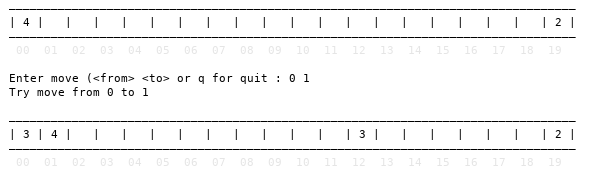
\includegraphics[width=.9\linewidth]{img/out-1.png}

\begin{itemize}

	\item Le jeu est initialisé de manière aléatoire avec les deux billes
		\textcircled{\tiny 4} et \textcircled{\tiny 2} aux positions
		respectives, 0 et 19\footnote{Le fait que ce soit au début et à la fin
		est du au hasard.}.

	\item Le joueur déplace la bille \textcircled{\tiny 4} de la position
		0 à la position 1 et deux billes aux valeurs aléatoires sont ajoutées
		à des positions aléatoires ce qui donne le deuxième état du jeu pour cet 
		exemple.

\end{itemize}

\clearpage
\textbf{Exemple d'une suppression de 3 billes identiques}

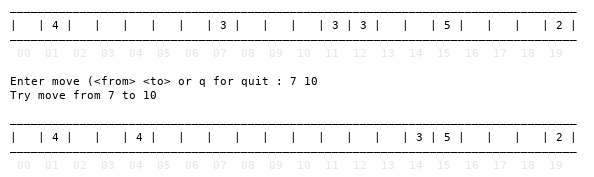
\includegraphics[width=.9\linewidth]{img/out-2.png}

\begin{itemize}

	\item Le déplacement de la bille \textcircled{\tiny 3} en position 7 vers
		la position 10 est autorisé. Ce déplacement a pour effet d'aligner
		3 billes de mêmes valeurs aux positions contigües 10, 11 et 12.  

	\item Les billes étant : trois, de même valeur et contigües, elles 
		disparaissent. 

	\item Après chaque déplacement, deux nouvelles billes de valeur aléatoire
		et à une position aléatoire apparaissent. Il s'agit, dans cet exemple,
		des billes de valeur \textcircled{\tiny 3} et \textcircled{\tiny 4} aux
		positions respectives 14 et 4.  

\end{itemize}



\begin{infoit}{Choix techniques}
	\begin{enumerate}
		\item Le plateau de jeu est représenté par un tableau d'entiers de 
			taille 20. 
		\item Les billes sont représentées par un entier numéroté de 1 à 5. 
		\item Une case vide est représentée par l'entier 0. 
		\item La classe s'appellera \texttt{g12345.inline.InLine}. Elle fait donc
			partie du package \texttt{g12345.inline}, s'appelle \texttt{InLine} et 
			se trouve dans un fichier \texttt{InLine.java}. 
	\end{enumerate}
\end{infoit}


\bigskip
\begin{infobox}
	Pour l'exercice, vous aurez besoin d'un dépôt \textit{git}. Vous pouvez
	travailler dans votre dépôt habituel contenant tous les exercices de vos
	tds ou en créer un pour l'occasion. À votre meilleure convenance. 
\end{infobox}

\bigskip


\section{Déplacer une bille (version 1)}

La méthode \code{java}{move} qui déplace une bille a besoin comme paramètres en
entrée~: le plateau de jeu représenté par un tableau d'entiers, un entier pour
la position de départ et un entier pour la position d'arrivée. 

Voici la signature de la méthode~:

\begin{Code}{java}
	public static void move(int[] is, int from, int to)
\end{Code}

Il s'agira bien d'écrire une méthode qui déplace un élément dans un tableau
d'entiers. 

\pagebreak
\begin{Exercice}{Écrire les tests}
	Commençons par demander à Netbeans de générer de code pour nous. 

	\begin{steps}		
		\item Dans la classe \texttt{InLine} ajoutez la méthode \texttt{move}
			qui ne fait rien pour l'instant et d'un clic droit, demandez
			à Netbeans de générer les tests pour cette méthode. 

		\item Écrivez des tests pour cette méthode.
	\end{steps}

Dans votre plan de tests, pensez à~:

\begin{itemize}
	\item un cas général où il n'y a pas de billes sur le chemin;
	\item un cas général où il y a une bille sur le chemin;
	\item un cas où la position de départ est hors tableau;
	\item un cas où la position de départ ne contient pas de bille;
	\item un cas où la position d'arrivée est hors tableau;
	\item un cas où la position d'arrivée contient déjà une bille;
	\item un cas où il y a plus d'une bille sur le chemin.
\end{itemize}

\end{Exercice}

Lancez vos tests… et constatez qu'ils échouent tous. C'est normal. Continuons. 

\begin{Exercice}{Écrire la première version}
	\begin{steps}
		\item Écrivez la méthode \texttt{move} pour qu'elle déplace une bille
			sans se soucier de savoir combien de billes se trouvent entre la
			position de départ et la position d'arrivée. Votre méthode
			vérifiera par contre que le mouvement reste bien dans le tableau,
			qu'il y a une bille à la position de départ et que la position 
			de destination n'est pas occupée. 

		\item Lancez vos tests. Les six premiers tests doivent réussir. Le
			dernier sera pour plus tard.
	
\end{steps}
\end{Exercice}

\findefonctionnalite




\section{Quelques méthodes simples}

\begin{Exercice}{Ajouter deux billes}
	\begin{steps}
		\item Écrivez une méthode \texttt{add2bals} ajoutant deux billes à deux 
			endroits libres aléatoires du tableau de jeu. 
	\end{steps}

	Vous ne devez pas tester cette méthode mais bien écrire la javadoc. 

	Voici la signature de la méthode~:

	\begin{Code}{java}
		public static void add2bals(int[] is)
	\end{Code}

	\paragraph{Remarque~:} Soyez attentif au fait que vous ne pourrez pas placer 
	deux billes sur le tableau de jeu si celui-ci ne contient plus deux places 
	libres. C'est donc mieux de vérifier à un moment donné. 

\end{Exercice}

\begin{Exercice}{Afficher le tableau de jeu}
	\begin{steps}
		\item Écrivez une méthode \texttt{display} qui affiche le tableau de jeu. 
	\end{steps}

	Affichez un espace lorsqu'il n'y a pas de bille et la valeur de la bille
	lorsqu'une bille est présente. 

	Vous ne devez pas tester cette méthode mais bien écrire la javadoc.

	Voici la signature de la méthode~:
	\begin{Code}{java}
		public static void display(int[] is)
	\end{Code}

\end{Exercice}

\findefonctionnalite



\section{Retirer des billes}

La méthode \code{java}{remove3inline} parcourt le tableau de jeu et retire les
billes dès lors qu'il y a trois billes de même couleurs côte à côte. 

L'algorithme est un peu compliqué, il s'agit de chercher une suite de trois
entiers identiques dans un tableau d'entiers. Mieux vaut y réfléchir un peu sur
papier avant de se lancer tête baissée. 

Voici la signature de la méthode~:
\begin{Code}{java}
	public static void remove3inline(int[] is)
\end{Code}

\begin{Exercice}{Écrire les tests}
	Redemandons à Netbeans de générer les tests pour nous.
	\begin{steps}		
		\item Dans la classe \texttt{InLine} ajoutez la méthode 
			\texttt{remove3inline}
			qui ne fait rien pour l'instant et d'un clic droit, demandez
			à Netbeans de générer les tests pour cette méthode. 

		\item Écrivez des tests pour cette méthode.
	\end{steps}

	Cette fois, nous vous laissons réfléchir à votre plan de tests. Une fois
	vos tests écrits… ne les lancez pas. Ils échoueront ;-)

\end{Exercice}

\begin{Exercice}{Écrire la méthode}
	Après avoir réfléchis à l'algorithme sur papier : 
	\begin{steps}
	\item écrivez la méthode \texttt{remove3inline}.
	\item Lancez vos tests. 
	\end{steps}
\end{Exercice}

\findefonctionnalite 



\section{Interface}

Tout est en place pour écrire l'interface utilisateur et utilisatrice. Il
s'agit de demander à l'utilisateur ou à l'utilisatrice quel mouvement iel veut
faire et tant qu'iel ne désire pas s'arrêter, continuer. 

Nous ne traiterons pas ici du tableau de jeu rempli ou ne permettant plus de
faire un déplacement. 

\begin{Exercice}{Écrire l'interface}
	\begin{steps}
	\item Écrivez une méthode robuste de demande du mouvement ou de fin.
	\item Écrivez une méthode \texttt{main} permettant de jouer au jeu. En voici 
		les étapes principales~:
		\begin{itemize}
			\item créer le tableau de jeu (le tableau d'entiers);
			\item l'initialiser avec deux billes placées aléatoirement (via la 
				méthode \texttt{add2bals});
			\item dans une boucle~: lire le mouvement désiré, 
				l'appliquer (via la méthode \texttt{move}) s'il est valide, 
				ajouter deux billes placées aléatoirement
				(via la méthode \texttt{add2bals},
				vérifier si trois billes sont en lignes et les supprimer 
				(via la méthode \texttt{remove3inline})\footnote{Le choix est 
				fait d'ajouter d'abord les billes supplémentaires avant de 
				supprimer les triplets pour le cas où une des deux billes 
				supplémentaires serait une troisième.}; 
			\item signaler la fin du jeu et quitter. 
		\end{itemize}
	\end{steps}
\end{Exercice}

\findefonctionnalite 

\section{Déplacer une bille (version 2)}

Notre première version du déplacement ne vérifiait pas le nombre de bille entre
la position de départ et la position d'arrivée. Il est temps d'ajouter cette
dernière fonctionnalité. 

\begin{Exercice}{Écrire la méthode \texttt{move} (version 2)}
	\begin{steps}
	\item Revoyez la méthode \texttt{move} pour qu'elle gère correctement le 
		déplacement. 
	\item Relancez vos tests qui devraient tous réussir maintenant. 
	\end{steps}
\end{Exercice}

\findefonctionnalite 

\section{Conclusion}

Pour arriver au terme de cet exercice, c'est normal d'y consacrer deux heures au 
laboratoire et deux heures en dehors. 

Bien qu'une solution soit fournie, nous espérons que vous avez pu mener à bien
l'exercice sans la consulter. La solution fournie, n'est pas parfaite, le mieux
pour vous est de demander un retour sur \textbf{votre} code à votre enseignant
ou enseignante. 




\end{document}
